%!TEX TS-program = pdflatex
\documentclass{emulateapj}

\shorttitle{AQS on MIKE}
\shortauthors{Casey et al}

\begin{document}

\title{The Aquarius Stream Progenitor Was Not A Globular Cluster: \\ Its History is Far More Interesting}


\author{Andrew R. Casey\altaffilmark{1,2} and distinguished collaborators}
\altaffiltext{1}{Research School of Astronomy \& Astrophysics, Australian National University, Mount Stromlo Observatory, via Cotter Rd, Weston, ACT 2611, Australia}
\altaffiltext{2}{Massachusetts Institute of Technology, Kavli Institute for Astrophysics and Space Research,
77 Massachusetts Avenue, Cambridge, MA 02139, USA}


\begin{abstract}
\end{abstract}

\keywords{Galaxy: halo, structure --- Individual: Aquarius Stream --- Stars: FGK-giants}

\section{Introduction}

Stellar streams in the halo are relics from relatively recent minor mergers in the Milky Way. The positions and kinematics of stars within these streams are sensitive to the galactic potential. As such, they can collectively constrain the fraction and distribution of accreted matter in the stellar halo, the sub-halo mass function, as well as the shape and extent of dark matter in the Milky Way. Moreover, individual elemental abundances for stars within these streams reveal the chemodynamical evolution of the Galaxy. 

Wide-field surveys have proved excellent sources for finding stellar streams. Dozens of streams reaching out up to 150\,kpc in the stellar halo have been identified through photometric selections and matched-filtering techniques. However, as \citet{Helmi;White_1999} point out, these methods are only successful for identifying substructures that are sufficiently distant from the solar neighbourhood. A nearby stream within $\sim{}$10\,kpc will not appear as an on-sky over-density. Such substructures would only be detectable by utilising both position and kinematic information. 

% Talk about RAVE
It is therefore necessary to survey the kinematics of solar neighbourhood stars in order to detect nearby streams. The RAVE (Radial Velocity Experiment) began such a survey in 2003 and has observed spectra from over 500,000 stars across 17,000 deg$^{2}$. RAVE candidates were photometrically selected based only on their apparent magnitude of 9 $<$ I $<$ 13, and are therefore kinematically unbiased. The RAVE data releases have provided radial velocities \citep{steinmetz;et-al_2006} and estimates of stellar parameters \citep{zwitter;et-al_2008, siebert;et-al_2011} now for a subset of these observations. 

% Identification of the aquarius stream
Using this data, \citet{williams;et-al_2011} identified a co-moving group of nearby ($0.5 \lesssim d \lesssim 10$\,kpc) stars in the direction of the Aquarius constellation. The artefact is most apparent when examining kinematics against galactic latitude for stars within $-70\,^\circ < b < -50\,^\circ$. \citet{williams;et-al_2011} employed a selection criteria of $-250 < V_{hel} < -150$\,km s$^{-1}$, $30\,^\circ < l < 75\,^\circ, J > 10.3$ and identified 15 stream candidates. The average heliocentric radial velocity of these members was found to be $V_{HELIO} = -199$\,km s$^{-1}$, with a dispersion of 27\,km s$^{-1}$. When compared to other streams identified in the halo, this is an unusually wide kinematic dispersion. Streams are generally considered to be kinematically cold, with dispersions of $\sigma_v < 8$\,km s$^{-1}$. The radial velocities outputted by the RAVE survey are described to be $\sim2$\,km s$^{-1}$, so the wide kinematic distribution appears to be real.

% is it a real substructure
\citet{williams;et-al_2011} quantified the statistical significance of the Aquarius substructure with comparisons to the Besancon and Galaxia models. After populating the models, the galaxy representations were discretized in $\Delta{}V_{hel}$ and $\Delta{}l$ grid blocks. 

There is no reason to suspect that the Aquarius stream is not a real substructure.

% What is it?
Given the extent of stellar debris the Sagittarius dwarf has littered in the Milky Way, it is reasonable to suspect the Aquarius stream might be Sagittarius in origin. Although the metallicities reported by \citet{williams;et-al_2011} are not dissimilar from the stream, the distances and $V_{Z}$, $V_\phi$ for Aquarius are quite distinct from Sagittarius. \citet{williams;et-al_2011} concluded that the newly discovered stream could not be positively associated with the Monoceros stream, Hercules-Aquila cloud, or either the Canis Major or Virgo Overdensities.

% MRS follow-up by de boer
In order to investigate the Aquarius progenitor and any possible association with existing substructures, \citet{wylie-de-boer;et-al_2012} observed six Aquarius stream members with medium resolution (R = 25,000) spectroscopy. Their data indicates the stream is chemically coherant, with a dispersion in [Fe/H] of only 0.1\,dex. This minimal chemical scatter suggests that the Aquarius stream progenitor is a globular cluster, since dwarf spheroidal galaxies  exhibit chemical dispersions of a dex or more \citet{Frebel_Norris_2011}. 

 Based on sodium and nickel abundance ratios with respect to iron, they claim the Aquarius stream chemical signatures unambiguously represent those of a globular cluster.
 
% globular cluster chemical signatures

We seek to investigate the globular cluster origin claim made by \citet{wylie-de-boer;et-al_2012}. We present a detailed chemical abundance analysis for five confirmed Aquarius stream members observed using the Magellan Inamori Kyocera Echelle spectrograph \citep{Bernstein;et-al_2003} on the Magellan telescope. Details of the observations and data reduction are outlined in the following section. The data analysis is presented in \S\ref{sec:analysis} and a detailed discussion of these results resides in \S\ref{sec:discussion}. In \S\ref{sec:conclusion} we present our conclusions and critical interpretations.

\section{Observations \& Data Reduction}

The most comprehensive sample of Aquarius stream stars is presented in the discovery paper of \citet{williams;et-al_2011}. Since the globular cluster origin claim of \citet{wylie-de-boer;et-al_2012} is based from a subset of six of these stars, we targeted stars largely from this study. Four of our stars are in common with \citet{wylie-de-boer;et-al_2012}. An additional star from the original \citet{williams;et-al_2011} sample, J2306265-085103, was also observed. J2306265-085103 had insufficient S/N for the RAVE pipeline to accurately determine stellar parameters, so its membership hinges on radial velocity measurements. Program stars were observed in July 2011 and we observed X standard stars observed for a separate program in March 2011. All observations were taken using the 1.0" slit, which provides a spectral resolution of $R = 28,000$. The exposure times for our program stars varied per star from X seconds to Y seconds to ensure a signal-to-noise in excess of 100 per pixel element at 600 nm for all stars.

The data were reduced using the CarPy pipeline. Standard flat-fielding and extraction methods were employed using 10 quartz and 10 milky frames taken at the start of each night. ThAr arc lamp exposures were taken at the start of each night to provide wavelength calibration. No telluric corrections were made as atmospheric absorption does not affect any of the transitions in our line list. Each reduced echelle order was carefully normalised using a third order spline. All normalised orders were stitched together to provide a single one-dimensional spectrum from 3800-9400\,\AA{}. 

\begin{deluxetable*}{lcccccccccc}
\tablecolumns{1}
\tabletypesize{\scriptsize}
\tablecaption{Observations\label{tab:observations}}
\tablehead{
	\colhead{Designation} &
	\colhead{$\alpha$} &
	\colhead{$\delta$} &
	\colhead{Observed} &
	\colhead{Airmass} &
	\colhead{Seeing} &
	\colhead{$t_{exp}$} &
	\colhead{S/N\tablenotemark{a}} &
	\colhead{$V_{rad}$} &
	\colhead{$V_{hel}$} &
	\colhead{$V_{err}$} \\
 & (J2000) & (J2000) & Date & & (") & (secs) & (px$^{-1}$) & (km s$^{-1}$) & (km s$^{-1}$) & (km s$^{-1}$)
}
\startdata

C2225316-14437	& 22:25:31.7 & $-$14:54:39.6	& 2011-07-30	& 1.033 & \dots & \dots & \dots & $-$169.0	& \dots & 0.7 \\
C2306265-085103	& 23:06:26.6 & $-$08:51:04.8	& 2011-07-30	& 1.096 & \dots & \dots & \dots & $-$239.3	& \dots & 0.6 \\
HD41667			& 06:05:03.7 & $-$32:59:36.8	& 2011-03-13	& 1.005	& \dots & \dots & \dots & 314.4	& \dots & 0.8 \\
HD142948		& 16:00:01.6 & $-$53:51:04.1	& 2011-03-14	& 1.107	& \dots & \dots & \dots & 6.8		& \dots & 0.4 \\
J221821-183424	& 22:18:21.2	& $-$18:34:28.3	& 2011-07-30	& 1.026	& \dots & \dots & \dots & $-$170.5	& \dots & 0.5 \\
J223504-152834	& 22:35:04.5	& $-$15:28:34.9	& 2011-07-30	& 1.047	& \dots & \dots & \dots & $-$180.9	& \dots & 0.7 \\
J223811-104126	& 22:38:11.6	& $-$10:41:29.4	& 2011-07-30	& 1.218	& \dots & \dots & \dots & $-$248.4	& \dots & 0.7 

\enddata
\tablenotetext{a}{S/N measured at 6000 \AA{} for each target.}
\end{deluxetable*}


\section{Analysis}
\label{sec:analysis}

\subsection{Radial Velocities}
\label{sec:radial-velocities}
The radial velocity for each star was determined in a two-step method. An initial estimate of the radial velocity was ascertained by cross-correlation with a synthetic spectrum of a giant with $T_{eff} = 4500$\,K, $\log{g} = 1.5$, and [M/H] $= -1.0$ across the wavelength range $8450 - 8700$ \AA{}. The spectrum was shifted to rest frame using this initial velocity. Velocities found from cross-correlation are typically within 1\,km\,s$^{-1}$ of our final published value.

With our spectrum at near-rest, we measured the equivalent widths of $N$ lines by fitting Gaussian functions to the absorption profiles. Fitting Gaussian profiles provides us with the measured equivalent width, the full-width half-maximum of the profile, and the central wavelength. Thus, the residual radial velocity can be found from the ratio of the central and rest line wavelengths. The final radial velocity for the star is provided by the mean of these $N$ line velocity measurements. Figure \ref{fig:line-velocities} shows the line velocities for HD41667 after  being placed at rest using our cross-correlation velocity of 314.4\,km s$^{-1}$. As expected, the mean offset is small ($-0.75$\,km s$^{-1}$), and our standard deviation is 0.79\,km s$^{-1}$ from 164 line measurements. This provides us with a final measured radial velocity of $313.7 \pm 0.1$\,km s$^{-1}$. This process was repeated for all observations. The radial velocities published in Table \ref{tab:observations} are the final values from this two-step method. Heliocentric velocities agree excellently (within X\,km s$^{-1}$) with previously reported literature values \citep{williams;et-al_2011,wylie-de-boer;et-al_2012}.

\begin{figure}[h]
	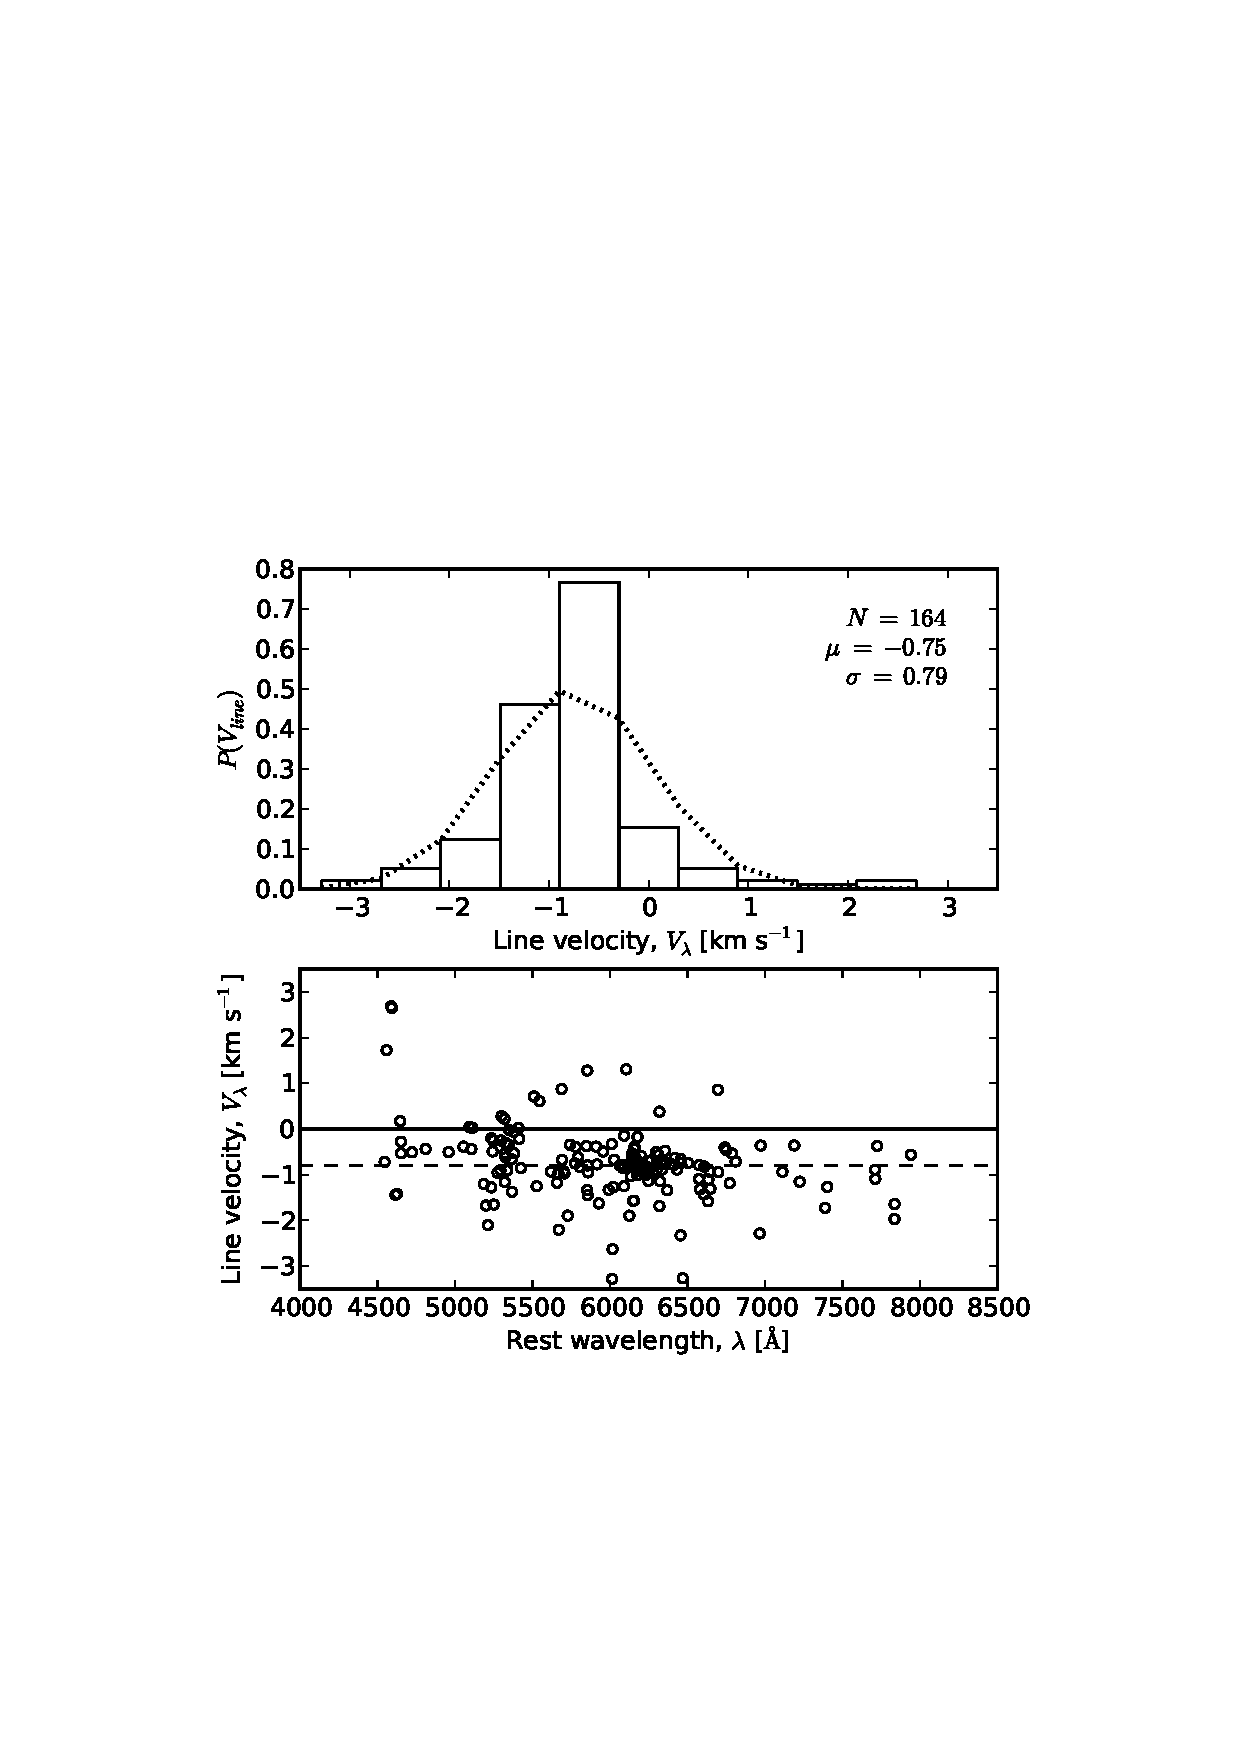
\includegraphics[width=\columnwidth]{./figures/line-velocity.pdf}
	\caption{Line velocity measurements.}
	\label{fig:line-velocities}
\end{figure}

\subsection{Line Measurements}
\label{sec:line-measurements}

For the measurement of atomic absorption lines, we employed the line list of \citet{yong;et-al_2005} with additional transitions of Cr, Sc, Zn, and Sr from \citet{frebel;et-al_2010}. We supplemented the list with hyperfine-structure data for Sc and Mn from the Kurucz compilation \citet{Kurucz;1998}. Molecular line data for CH was taken from \citet{Plez;et-al_2008,Plez;et-al_2009}. For lines with hyperfine structure, blended transitions or molecular features, we determined the transition abundance using a spectral synthesis approach where the abundance of a given species is found by by matching a synthetic spectrum to the observed spectrum.

The equivalent widths for all transitions were measured automatically using software for this study. Given the rest wavelength and an initial guess of the FWHM, a Gaussian function is iteratively fitted to the absorption profile. At the same time, the local continuum is found within 20\,\AA{} either side of the rest wavelength using a second-order polynomial. Measuring the local continuum ensures any errors in our initial normalisation or order-stitching do not propagate through to our equivalent width measurements. Any group of pixels that deviate significantly ($>2\sigma$) to the local continuum are cosmic ray hits, or more likely trough points of a neighbouring profile. We attempt to fit a Gaussian profile to each of these groups of deviating pixels, using the best estimate of the local continuum. If a profile is successfully fitted, then all points belonging to that profile are excluded from the continuum determination. When fitting Gaussian profiles, the $\chi^2$ difference between the observation and the profile is minimized. In order to account for blended transitions, our $\chi^2$ function is weighted based on the distance to the rest wavelength. Pixels near the rest wavelength are weighted higher than those on the wings. Although this approach relies on an accurate ($<4$\,km s$^{-1}$) radial velocity correction, it greatly improves the accuracy of the equivalent width measurements.

We note that the results of our iterative fitting approach are entirely insensitive to the initial FWHM guess. Increasing the initial guess from 0.1\,\AA{} to 1 or 2\,\AA{} -- an unphysical large value for high-resolution spectra -- does not alter our equivalent width measurements. Only a small increase in computational cost is observed. Although we are confident in our automatic equivalent width measurements, every absorption profile was examined by eye for quality. 

We list the atomic data and measured equivalent widths for atomic lines used during this analysis in Table \ref{tab:equivalent-widths}. Saturated lines were excluded by removing measurements with reduced equivalent widths, $\log_{10}{(EW/\lambda)} > -4.5$\, dex. A minimum detectable equivalent width was calculated as a function of wavelength based on the S/N, and only lines that exceeded a $3\sigma$ detection significance were included. We have verified our equivalent width measurement techniques by comparing our measurements for 164 lines in HD140283 with the study of \citet{Norris;et-al_1996}. Excellent agreement is found between the two studies, which is illustrated in Figure \ref{fig:ew-compare}. The mean difference between this study and that of \cite{norris;et-al_1996} is a negligible $0.64 \pm 2.78$\,m\AA{}, and no systematic trend is present.

% equivalent widths plot with Norris for HD 122563
\begin{figure}[h]
	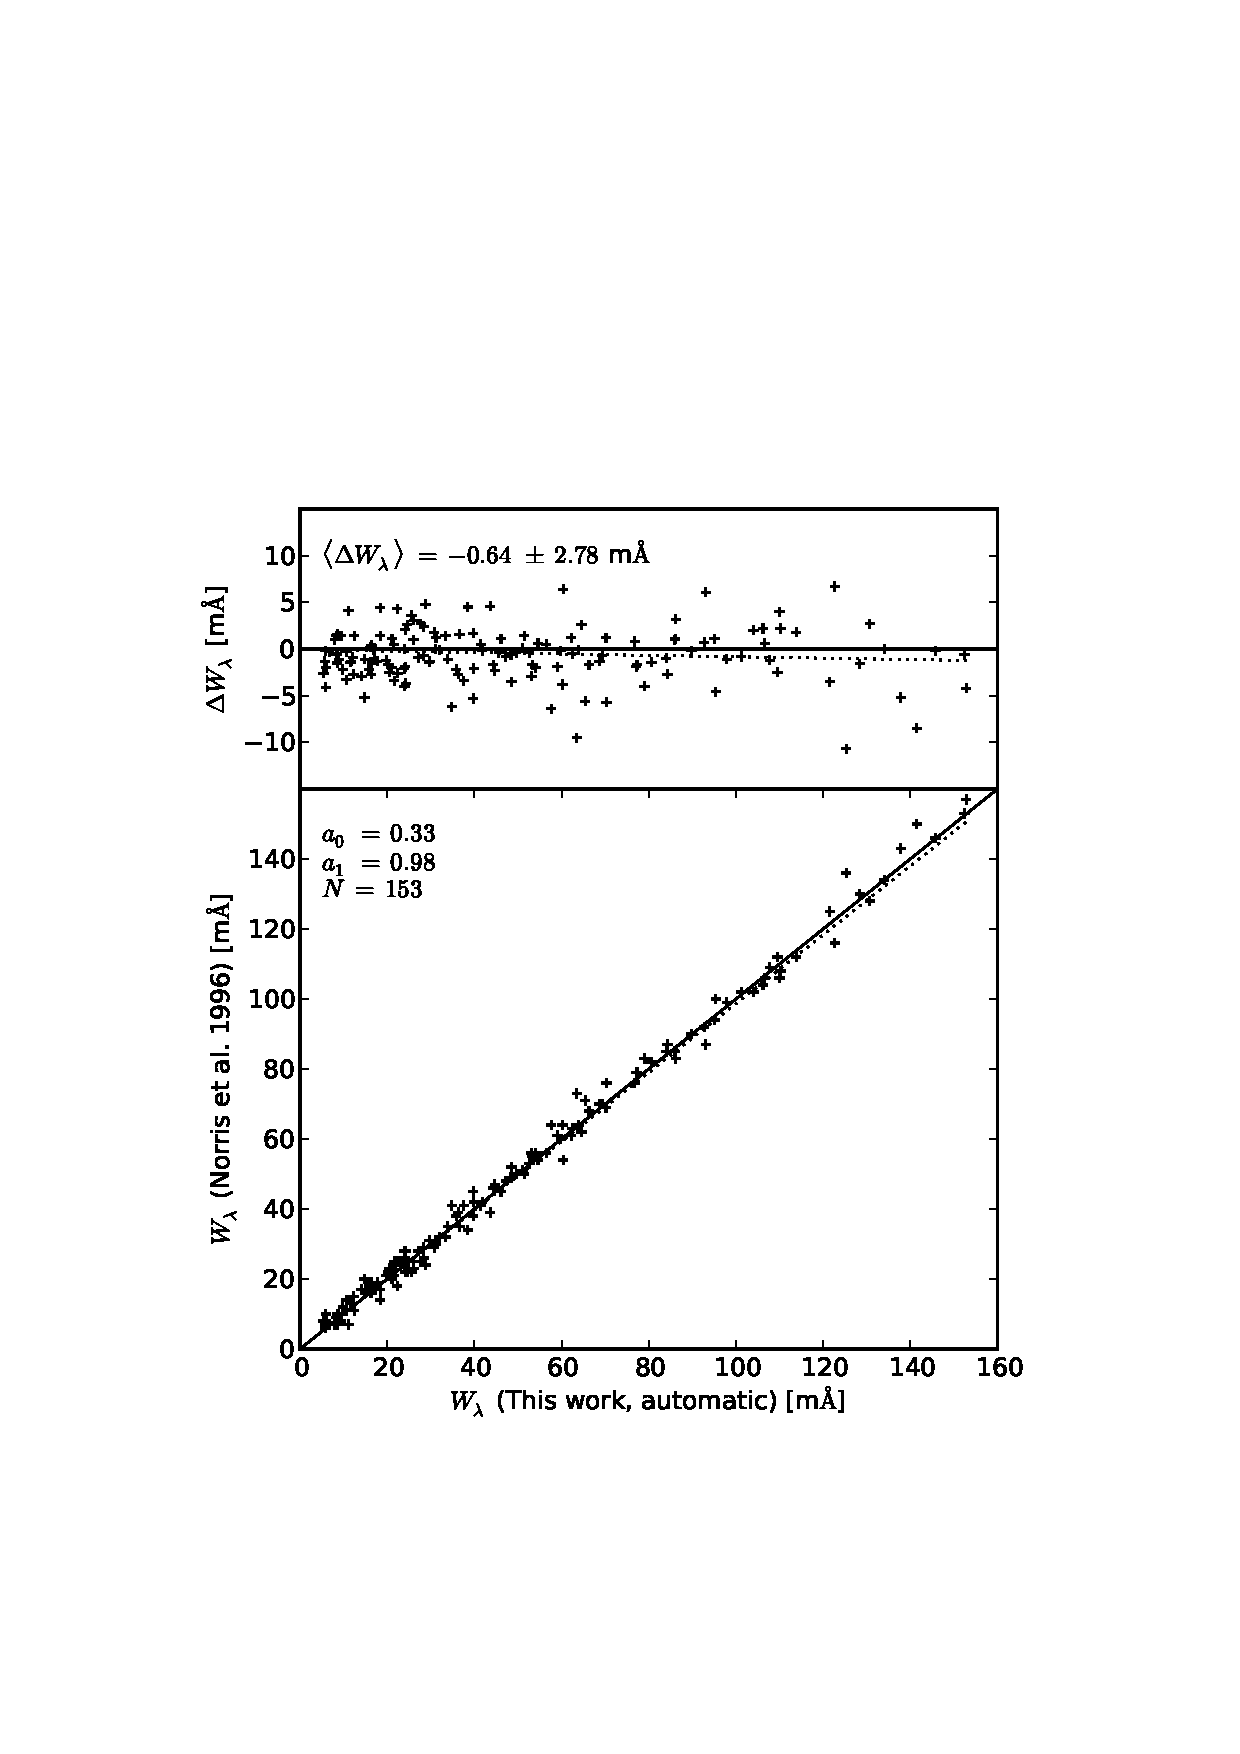
\includegraphics[width=\columnwidth]{./figures/smh-norris.pdf}
	\caption{The gold standard comparison.}
	\label{fig:ew-compare}
\end{figure}

% equivalent widths table

\subsection{Model Atmospheres}
We employed the ATLAS9 stellar atmospheres of \citet{Castelli;Kurucz_2003} for this analysis. These one-dimensional models ignore any centre-to-limb spatial variations, assume hydrostatic equilibrium and no convective overshoot from the photosphere. Absorption lines are assumed to form under the assumption of local thermal equilibrium. The stellar parameter spacing for these grid models is 250\,K, 0.5 dex in surface gravity, 0.5 dex in [M/H] and 0.1 dex in [$\alpha$/Fe]. We interpolated the atmospheric densities, temperatures, electron pressures at all depths between stellar atmospheres using the Quickhull algorithm for this analysis. Quickhull is reliant on Delaunay tessellation, which suffers from extremely skewed cells when the grid points vary in size by orders of magnitude -- as $T_{eff}$ values do compared to $\log{g}$ or [X/H]. If unaccounted for, these asymmetric cells can manifest as significant errors in interpolated densities, temperatures, pressures, and opacities across all photospheric depths. We scaled each stellar parameter between zero and unity prior to interpolation to minimise these errors. During this step, $\log{g}$, [Fe/H] and [$\alpha$/Fe] points were scaled such that we simultaneously interpolate linearly in $T_{eff}$ and logarithmically in all other parameters.

\subsection{Stellar Parameters}
The most recent version of the spectral synthesis code MOOG \citep{Sneden;et-al_1973} has been used to derive individual line abundances and stellar parameters. This version employs a more accurate treatment of Rayleigh scattering \citep{Sobeck;et-al_2011}, which is particularly important for transitions blueward of 450\,nm. This is noteworthy, but is less relevant for this analysis as most of our line measurements are redward of 450\,nm. We have scaled our abundances to solar values using the chemical composition of \citet{Asplund;et-al_2009}.

The effective temperature for each star was found by demanding a zero-trend in excitation potential and abundance for each measured Fe\,I line. In the same way, the microturbulence was found by demanding a zero trend in reduced equivalent width against abundance. Linear relationships with slopes of $|0.001|$ dex were considered to be converged. Surface gravity was found by forcing the mean Fe\,I and Fe\,II abundances to be equal, whilst maintaining zero trends with the excitation potential, reduced equivalent width and abundance. After these parameters had converged, the model metallicity was exactly matched to that of our line abundances. Line abundances that were unusually deviant ($>3\sigma$) from the mean were removed. The largest number of outlier measurements removed for any observation was N for X.


% spectral plots for five stars

\begin{deluxetable*}{lcccccccccccccc}
\tablecolumns{2}
\tabletypesize{\scriptsize}
\tablecaption{Stellar Parameters}
\tablehead{
	\colhead{Designation} &
	\colhead{$T_{\mbox{eff}}$} &
	\colhead{$\log{g}$} &
	\colhead{$v_t$} &
	\colhead{[Fe/H]} & 
	\colhead{$T_{\mbox{eff}}$} &
	\colhead{$\log{g}$} &
	\colhead{$v_t$} &
	\colhead{[Fe/H]} &
	\colhead{Source} \\
}
\startdata
C2225316-14437	& 4350	& 1.60	& 1.80	& --1.19	
				& 4235 $\pm$ 118 & 1.45 $\pm$ 0.21 & 1.96 $\pm$ 0.11 & --1.20 $\pm$ 0.14 
				& \citet{wylie-de-boer;et-al_2012} \\
C2306265-085103	& 4180	& 1.00	& 1.80 	& --1.16
				& \dots	& \dots	& \dots	& \dots
				& \dots \\	
HD41667			& 4630	& 1.70	& 1.66 	& --1.21
				& 4605	& 1.88	& 1.44	& --1.16
				& \citet{Gratton;et-al_2000} \\
HD44007			& 4790	& 1.78	& 1.63	& --1.80
				& 4850	& 2.00 	& 2.20	& --1.71
				& \citet{Fulbright_2000} \\
HD142948		& 4950	& 2.19	& 1.78	& --0.79
				& 4713 	& 2.17 	& 1.38	& --0.77
				& \citet{Gratton;et-al_2000} \\
J221821-183424	& 4570	& 0.80	& 1.93	& --1.60
				& 4395 $\pm$ 205 & 1.45 $\pm$ 0.35 & 1.96 $\pm$ 0.18 & --1.15 $\pm$ 0.21
				& \citet{wylie-de-boer;et-al_2012} \\
J223504-152834	& 4620	& 2.15 	& 1.44	& --0.65
				& 4597 $\pm$ 158 & 2.40 $\pm$ 0.14 & 1.47 $\pm$ 0.07 & --0.98 $\pm$ 0.17
				& \citet{wylie-de-boer;et-al_2012} \\
J223811-104126	& 5100	& 3.00	& 1.21	& --1.44
				& 5646 $\pm$ 147 & 4.60 $\pm$ 0.15 & 1.09 $\pm$ 0.11 & --1.20 $\pm$ 0.20
				& \citet{wylie-de-boer;et-al_2012} 
\enddata

\end{deluxetable*}


\subsection{Abundances}


\begin{deluxetable*}{lccccccclcccccc}
\tablecolumns{15}
\tablecaption{Program Star Abundances\label{tab:program-star-abundances}}
\tablehead{
 \multicolumn{7}{c}{J221821-183424} & \colhead{} & \multicolumn{7}{c}{C2225316-14437} \\
 \cline{1-7} \cline{9-15} \\
\colhead{Species} & $N$ & $\log\epsilon(X)$ & $\sigma_\epsilon$ & [X/H] & [X/Fe] & $\sigma$ &&
\colhead{Species} & $N$ & $\log\epsilon(X)$ & $\sigma_\epsilon$ & [X/H] & [X/Fe] & $\sigma$
}
\startdata
   O \textsc{I} &   2 &    7.50 &    0.04 & $-$1.18 &    0.41 &    0.02 &&
   O \textsc{I} &   2 &    7.90 &    0.01 & $-$0.79 &    0.48 &    0.01 \\
  Na \textsc{I} &   2 &    4.56 &    0.14 & $-$1.68 & $-$0.08 &    0.10 &&
  Na \textsc{I} &   3 &    5.09 &    0.17 & $-$1.15 &    0.12 &    0.10 \\
  Mg \textsc{I} &   4 &    6.55 &    0.37 & $-$1.04 &    0.55 &    0.18 &&
  Mg \textsc{I} &   4 &    6.98 &    0.24 & $-$0.62 &    0.65 &    0.12 \\
  Al \textsc{I} &   1 &    5.04 &    0.00 & $-$1.41 &    0.18 & \nodata &&
  Al \textsc{I} &   4 &    5.87 &    0.09 & $-$0.58 &    0.68 &    0.04 \\
  Si \textsc{I} &   5 &    6.28 &    0.08 & $-$1.23 &    0.37 &    0.04 &&
  Si \textsc{I} &   5 &    6.96 &    0.15 & $-$0.55 &    0.72 &    0.07 \\
  Ca \textsc{I} &   4 &    4.97 &    0.04 & $-$1.37 &    0.23 &    0.02 &&
  Ca \textsc{I} &   4 &    5.50 &    0.04 & $-$0.84 &    0.43 &    0.02 \\
  Sc \textsc{I} &   0 & \nodata & \nodata & \nodata & \nodata & \nodata &&
  Sc \textsc{I} &   0 & \nodata & \nodata & \nodata & \nodata & \nodata \\
 Sc \textsc{II} &   6 &    1.52 &    0.08 & $-$1.63 & $-$0.04 &    0.03 &&
 Sc \textsc{II} &   5 &    2.05 &    0.13 & $-$1.10 &    0.17 &    0.06 \\
  Ti \textsc{I} &   0 & \nodata & \nodata & \nodata & \nodata & \nodata &&
  Ti \textsc{I} &   4 &    4.04 &    0.03 & $-$0.91 &    0.36 &    0.01 \\
 Ti \textsc{II} &   4 &    3.81 &    0.13 & $-$1.14 &    0.45 &    0.07 &&
 Ti \textsc{II} &   2 &    4.26 &    0.08 & $-$0.69 &    0.58 &    0.06 \\
   V \textsc{I} &   3 &    2.23 &    0.01 & $-$1.70 & $-$0.11 &    0.01 &&
   V \textsc{I} &   6 &    2.92 &    0.17 & $-$1.01 &    0.26 &    0.07 \\
  Cr \textsc{I} &  11 &    3.74 &    0.07 & $-$1.90 & $-$0.30 &    0.02 &&
  Cr \textsc{I} &   8 &    4.27 &    0.16 & $-$1.37 & $-$0.10 &    0.06 \\
  Mn \textsc{I} &   3 &    3.29 &    0.04 & $-$2.14 & $-$0.54 &    0.02 &&
  Mn \textsc{I} &   3 &    4.14 &    0.05 & $-$1.29 & $-$0.02 &    0.03 \\
  Fe \textsc{I} &  52 &    5.91 &    0.09 & $-$1.59 &    0.00 &    0.01 &&
  Fe \textsc{I} &  61 &    6.23 &    0.11 & $-$1.27 &    0.00 &    0.01 \\
 Fe \textsc{II} &  13 &    5.90 &    0.05 & $-$1.60 &    0.00 &    0.01 &&
 Fe \textsc{II} &  10 &    6.17 &    0.06 & $-$1.33 & $-$0.07 &    0.02 \\
  Co \textsc{I} &   1 &    3.35 &    0.00 & $-$1.64 & $-$0.05 & \nodata &&
  Co \textsc{I} &   3 &    3.92 &    0.12 & $-$1.07 &    0.20 &    0.07 \\
  Ni \textsc{I} &   5 &    4.61 &    0.15 & $-$1.61 & $-$0.01 &    0.07 &&
  Ni \textsc{I} &   7 &    5.04 &    0.09 & $-$1.18 &    0.09 &    0.03 \\
  Cu \textsc{I} &   1 &    2.13 &    0.00 & $-$2.06 & $-$0.47 & \nodata &&
  Cu \textsc{I} &   1 &    3.35 &    0.00 & $-$0.84 &    0.43 & \nodata \\
  Zn \textsc{I} &   2 &    3.15 &    0.11 & $-$1.41 &    0.19 &    0.08 &&
  Zn \textsc{I} &   2 &    3.46 &    0.23 & $-$1.10 &    0.17 &    0.17 \\
\cline{1-7} \cline{9-15} \\
\\
\multicolumn{7}{c}{J223504-152834} && \multicolumn{7}{c}{J223811-104126} \\
\cline{1-7} \cline{9-15} \\
   O \textsc{I} &   2 &    8.48 &    0.09 & $-$0.21 &    0.46 &    0.07 &&
   O \textsc{I} &   1 &    8.60 &    0.00 & $-$0.09 &    1.36 & \nodata \\
  Na \textsc{I} &   3 &    5.76 &    0.12 & $-$0.48 &    0.19 &    0.07 &&
  Na \textsc{I} &   2 &    4.76 &    0.10 & $-$1.48 & $-$0.03 &    0.07 \\
  Mg \textsc{I} &   3 &    7.50 &    0.24 & $-$0.10 &    0.58 &    0.14 &&
  Mg \textsc{I} &   3 &    6.49 &    0.42 & $-$1.11 &    0.34 &    0.24 \\
  Al \textsc{I} &   3 &    6.10 &    0.08 & $-$0.35 &    0.32 &    0.05 &&
  Al \textsc{I} &   2 &    5.10 &    0.14 & $-$1.35 &    0.10 &    0.10 \\
  Si \textsc{I} &   5 &    7.11 &    0.10 & $-$0.40 &    0.28 &    0.04 &&
  Si \textsc{I} &   3 &    6.38 &    0.04 & $-$1.13 &    0.32 &    0.02 \\
  Ca \textsc{I} &   4 &    6.03 &    0.04 & $-$0.31 &    0.36 &    0.02 &&
  Ca \textsc{I} &   4 &    5.30 &    0.03 & $-$1.04 &    0.41 &    0.01 \\
  Sc \textsc{I} &   0 & \nodata & \nodata & \nodata & \nodata & \nodata &&
  Sc \textsc{I} &   0 & \nodata & \nodata & \nodata & \nodata & \nodata \\
 Sc \textsc{II} &   6 &    2.70 &    0.14 & $-$0.45 &    0.23 &    0.06 &&
 Sc \textsc{II} &   6 &    1.75 &    0.14 & $-$1.40 &    0.05 &    0.06 \\
  Ti \textsc{I} &   4 &    4.63 &    0.02 & $-$0.32 &    0.36 &    0.01 &&
  Ti \textsc{I} &   0 & \nodata & \nodata & \nodata & \nodata & \nodata \\
 Ti \textsc{II} &   2 &    4.92 &    0.26 & $-$0.04 &    0.64 &    0.19 &&
 Ti \textsc{II} &   4 &    3.83 &    0.09 & $-$1.12 &    0.33 &    0.04 \\
   V \textsc{I} &   6 &    3.67 &    0.22 & $-$0.26 &    0.41 &    0.09 &&
   V \textsc{I} &   1 &    2.42 &    0.00 & $-$1.51 & $-$0.06 & \nodata \\
  Cr \textsc{I} &   7 &    4.94 &    0.09 & $-$0.70 & $-$0.02 &    0.03 &&
  Cr \textsc{I} &  12 &    4.12 &    0.06 & $-$1.52 & $-$0.07 &    0.02 \\
  Mn \textsc{I} &   3 &    5.08 &    0.10 & $-$0.35 &    0.33 &    0.06 &&
  Mn \textsc{I} &   3 &    3.55 &    0.04 & $-$1.88 & $-$0.43 &    0.02 \\
  Fe \textsc{I} &  64 &    6.83 &    0.12 & $-$0.67 &    0.00 &    0.02 &&
  Fe \textsc{I} &  33 &    6.05 &    0.06 & $-$1.45 &    0.00 &    0.01 \\
 Fe \textsc{II} &  12 &    6.82 &    0.07 & $-$0.68 &    0.00 &    0.02 &&
 Fe \textsc{II} &  11 &    6.00 &    0.09 & $-$1.50 & $-$0.05 &    0.03 \\
  Co \textsc{I} &   3 &    4.53 &    0.14 & $-$0.46 &    0.21 &    0.08 &&
  Co \textsc{I} &   0 & \nodata & \nodata & \nodata & \nodata & \nodata \\
  Ni \textsc{I} &   7 &    5.62 &    0.09 & $-$0.60 &    0.08 &    0.03 &&
  Ni \textsc{I} &   2 &    4.82 &    0.04 & $-$1.40 &    0.05 &    0.03 \\
  Cu \textsc{I} &   1 &    3.85 &    0.00 & $-$0.34 &    0.33 & \nodata &&
  Cu \textsc{I} &   1 &    2.39 &    0.00 & $-$1.80 & $-$0.35 & \nodata \\
  Zn \textsc{I} &   2 &    4.17 &    0.03 & $-$0.39 &    0.28 &    0.02 &&
  Zn \textsc{I} &   2 &    3.17 &    0.04 & $-$1.39 &    0.06 &    0.03 \\

\cline{1-7} \cline{9-15} \\
\\
\multicolumn{7}{c}{C2306265-085103} && \\
\cline{1-7} \\
   O \textsc{I} &   2 &    8.09 &    0.15 & $-$0.60 &    0.57 &    0.10 \\
  Na \textsc{I} &   2 &    5.25 &    0.00 & $-$0.99 &    0.18 &    0.00 \\
  Mg \textsc{I} &   2 &    6.84 &    0.07 & $-$0.76 &    0.41 &    0.05 \\
  Al \textsc{I} &   4 &    5.56 &    0.08 & $-$0.89 &    0.28 &    0.04 \\
  Si \textsc{I} &   5 &    6.66 &    0.08 & $-$0.85 &    0.32 &    0.03 \\
  Ca \textsc{I} &   4 &    5.48 &    0.04 & $-$0.86 &    0.31 &    0.02 \\
  Sc \textsc{I} &   0 & \nodata & \nodata & \nodata & \nodata & \nodata \\
 Sc \textsc{II} &   6 &    2.18 &    0.15 & $-$0.97 &    0.20 &    0.06 \\
  Ti \textsc{I} &   4 &    4.06 &    0.03 & $-$0.89 &    0.28 &    0.01 \\
 Ti \textsc{II} &   3 &    4.21 &    0.36 & $-$0.74 &    0.43 &    0.21 \\
   V \textsc{I} &   4 &    2.88 &    0.06 & $-$1.05 &    0.12 &    0.03 \\
  Cr \textsc{I} &   4 &    4.20 &    0.26 & $-$1.44 & $-$0.27 &    0.13 \\
  Mn \textsc{I} &   3 &    4.35 &    0.10 & $-$1.08 &    0.09 &    0.06 \\
  Fe \textsc{I} &  63 &    6.33 &    0.12 & $-$1.17 &    0.00 &    0.01 \\
 Fe \textsc{II} &  11 &    6.31 &    0.09 & $-$1.19 & $-$0.02 &    0.03 \\
  Co \textsc{I} &   3 &    4.00 &    0.15 & $-$0.99 &    0.18 &    0.08 \\
  Ni \textsc{I} &   7 &    5.08 &    0.08 & $-$1.14 &    0.03 &    0.03 \\
  Cu \textsc{I} &   1 &    3.55 &    0.00 & $-$0.64 &    0.53 &    0.00 \\
  Zn \textsc{I} &   2 &    3.38 &    0.14 & $-$1.18 & $-$0.01 &    0.10
\enddata
\end{deluxetable*}


% elemental abundances

% comparison to literature for a given star

% chemical synthesis


\subsection{Distances}
% isochrone fitting

% discuss Williams et al distances


\subsection{Dynamics}

% U, V, W calculations



\section{Discussion}

% RAVE pipeline discrepancies

% wylie de boer discrepancies

We seek to investigate the nature of the Aquarius stream, as well as the specific globular cluster origin claim by \citet{wylie-de-boer;et-al_2012}. The stellar parameters reported in \citet{wylie-de-boer;et-al_2012} differ slightly to those found in Table \ref{tab:stellar-parameters}. \citet{wylie-de-boer;et-al_2012} deduce their stellar parameters through the use of a $\chi^2$ analysis against synthetic spectra from the \citet{munari;et-al_2005} grid. Our temperatures have been determined by forcing a zero trend in excitation potential and line abundance. In general, these temperatures agree within the uncertainties, with our temperatures being marginally (23-175 K) hotter. The only noteworthy exception is J223811-104126, where we find an effective temperature 546 K cooler than \citet{wylie-de-boer;et-al_2012}. This is the largest discrepancy we see in any of our standard or program stars. 


\citet{wylie-de-boer;et-al_2012} calculate microturbulence with the empirical relationships from \citet{Reddy;et-al_2003} for dwarfs and \citet{fulbright_2000} for giants. These relationships are based upon the derived temperature and surface gravities. Our published microturbulence values agree excellently with the values presented in \citet{wylie-de-boer;et-al_2012} with the exception of J223811-104126, which we find to be a F-type giant and others have claimed is a -type dwarf from medium-resolution spectra \citep{wylie-de-boer;et-al_2012, williams;et-al_2011}. Small discrepancies in microturbulence for other stars can be directly attributed to difference in surface gravities.


\subsection{Stellar Parameter Discrepancies with \citet{wylie-de-boer;et-al_2012}}

The stellar parameter discrepancies between this study and \citet{wylie-de-boer;et-al_2012} need to be addressed. There are noteworthy differences in the stellar parameter determination between these studies. In the \citet{wylie-de-boer;et-al_2012} study, the temperature, metallicity and surface gravity were found by a $\chi^2$ analysis against the spectral library of \citet{munari;et-al_2005} after it was convolved and re-sampled to match the observational data. The comparison regions used for analysis were 4900-5200\,\AA{} and 5575-5725\,\AA{}. Using these parameters, an interpolated MARCS (?) model atmosphere was used to synthesise elemental abundances. Oscillator strengths in their line list were astrophysical; they were derived from a reverse analysis using the \citet{hinkle;et-al_2003} solar atlas. The spectrum synthesis code \textsc{MOOG} was used to derive abundances for individual Fe\,I and Fe\,II lines. The median abundance of Fe\,I lines was taken as the overall stellar metallicity, scaled using the \citet{Grevesse;Sauval_1998} solar abundances.

The study of \citet{wylie-de-boer;et-al_2012} is of slightly lower resolution ($R = 25,000$ compared to $R = 28,000$ presented here), but with a much lower signal-to-noise ratio: $\sim{}25$ compared to $>100$ per pixel element achieved here. Given the slightly lower spectral resolution and modest signal-to-noise in their study, there are fewer unblended absorption lines available. In fact, there are very few transitions present in their published line list: only 14 Fe\,I lines and 3 Fe\,II lines are available. For contrast, our metallicity determinations are based off X Fe\,I and Y Fe\,II lines. Given the metallicity of these stars, it is somewhat surprising that there were not more unblended transitions available to \citet{wylie-de-boer;et-al_2012}.

With the exception of J223811-104126, we believe our stellar parameters are largely in agreement with the exception of metallicity. The Fe\,I abundances differ significantly for the four stars in common: 0.01\,dex, $-$0.45\,dex, 0.33\,dex, $-$0.24\,dex. In order to investigate the source of these discrepancies, we repeated our analysis for the four common stars using the line list of \citet{wylie-de-boer;et-al_2012}. The results of this analysis is shown in Table \ref{tab:wylie-de-boer-analysis-comparison}. 

One Fe\,I line at 6420.060\,\AA{} was not detectable in any of our stars, even though the S/N at this point exceeds 120 in every observation. Additionally, we could not identify the line in the existing VALD database.

% talk about stellar parameter differences

% we find their metallicities

Given the line list employed, the overall data quality and the lack of Fe\,I lines available for analysis, it appears the Aquarius stream stars have conspired to present a tight metallicity distribution function -- suggesting of a globular cluster origin. In contrast, our high-resolution analysis suggests a significantly broader metallicity distribution of $\langle$[Fe/H]$\rangle = X.XX \pm X.XX$ dex.

\subsection{The Aquarius Stream M.D.F.}

\subsection{The Na-O Relationship}

\subsection{The Al-Mg Relationship}

\subsection{The Na-Na Relationship}

\subsection{Possible Progenitors}

% Chemistries for various GC trends

% chemistries - [Na/O]

% chemistries - [Al/Mg]

% chemistries - [Ni/Na]


% closest looking globular clusters from Harris catalogue

% could they be displaced thick disk stars?


\begin{deluxetable*}{lccccccc}
\tablecolumns{2}
\tabletypesize{\scriptsize}
\tablecaption{Observed Targets\label{tab:observed-targets}}
\tablehead{
	\colhead{ID} &
	\colhead{$\alpha$} &
	\colhead{$\delta$} &
	\colhead{Air mass} &
	\colhead{S/N\tablenotemark{a}} &
	\colhead{$V_{\mbox{helio}}$} \\
 & (J2000) & (J2000) & & (px$^{-1}$) & (km s$^{-1}$)
}
\startdata


HD130694  			& 14:50:17.1 & --27:57:41.6 & 1.289 & \nodata & \nodata \\
HD170642  			& 18:32:21.0 & --39:42:12.8 & 1.464 & \nodata & \nodata \\
HD180928  			& 19:18:59.6 & --15:32:11.5 & 1.934 & \nodata & \nodata \\
HD181342  			& 19:21:03.9 & --23:37:09.7 & 1.203 & \nodata & \nodata \\
HD187111 			& 19:48:39.3 & --12:07:17.8 & 1.281 & \nodata & \nodata \\
HD210049  			& 22:08:22.8 & --32:59:14.6 & 1.006 & \nodata & \nodata \\
C2225316-145437  	& 22:25:31.7 & --14:54:39.6 & 1.033 & \nodata & \nodata \\
J221821-183424 		& 22:18:21.2 & --18:34:28.3 & 1.026 & \nodata & \nodata \\
J223504-152834 		& 22:35:04.5 & --15:28:34.9 & 1.047 & \nodata & \nodata \\
J223811-104126 		& 22:38:11.6 & --10:41:29.4 & 1.218 & \nodata & \nodata \\
C2306265-085103		& 23:06:26.6 & --08:51:04.8 & 1.096 & \nodata & \nodata \\
HD219615  			& 23:17:10.7 &$+$03:16:51.9 & 1.412 & \nodata & \nodata 
\enddata
\tablenotetext{a}{S/N measured at 6000 \AA{} for each target.}
\end{deluxetable*}


%\facilities{Magellan:Clay}

\bibliographystyle{apj}
\bibliography{bibliography}

\end{document}
